\documentclass{beamer}

%% Load Latex packages
\usepackage{amssymb}
\usepackage{color}
\usepackage{float}
\usepackage[T1]{fontenc}
\usepackage{graphicx}
\usepackage{hyperref}
\usepackage[utf8]{inputenc}
\usepackage{lmodern}
\usepackage{makecell}
\usepackage[authoryear, round]{natbib}
\usepackage{ragged2e}
\usepackage{tikz} %% For drawing arrows
\usepackage{wrapfig}
\usepackage{xmpincl}
\usepackage{xspace}

%% Colors
%% ------
% Color panel used throughout the poster
\definecolor{lgray}{rgb}{0.9179688,0.9179688,0.9179688} % #ebebeb
\definecolor{dgray}{rgb}{0.796875,0.796875,0.796875} % #cccccc
\definecolor{vdgray}{rgb}{0.3984375,0.3984375,0.3984375} % #666666
\definecolor{coral}{rgb}{0.9960938,0.4960938,0.3125000} % #ff7f50
\definecolor{blue}{rgb}{0.4218750,0.6484375,0.8007812} % #6ca6cd
\definecolor{green}{rgb}{0.6992188,0.7265625,0.5078125} % #b3ba82
\definecolor{yellow}{rgb}{0.9570312,0.8671875,0.6992188} % #f5deb3


%% Coding fonts
%% ------------
%% Font for R chunks
\usepackage{listings}
\lstset{
  language=R,
  basicstyle=\tiny\ttfamily\color{vdgray}, % the size of the fonts that are used for the code
  numbers=left,                   % where to put the line-numbers
  numberstyle=\tiny\color{gray},  % the style that is used for the line-numbers
  stepnumber=1,                   % the step between two line-numbers.
  numbersep=0.1cm,                % how far the line-numbers are from the code
  backgroundcolor=\color{lgray},  % choose the background color. You must add \usepackage{color}
  deletekeywords={stat, model, matrix},
  keywordstyle=\color{blue},      % keyword style
  stringstyle=\color{green},      % string literal style
  xleftmargin=0.5cm,
}

%% Adapt template format 
%% ------------
%% headline
\setbeamercolor{section in head/foot}{bg=lgray, fg=black}
%% frametitle 
\setbeamerfont{frametitle}{series=\bfseries}
\setbeamercolor{frametitle}{bg=lgray, fg=black}
%% table of content
\setbeamercolor{section in toc}{fg=black}
\setbeamerfont{section in toc}{size=\large}
%% footer
\setbeamertemplate{footline}[text line]{
  \parbox{\linewidth}{
    \small
    \hfill
    \color{vdgray}{\insertframenumber}
    \hspace{-1cm}
    \vspace{0.3em}
  }
}
%% Remove the navigati
\beamertemplatenavigationsymbolsempty

%% Custom functions
%% ------------
%% Inline code highlight
\newcommand{\hcode}[2][lgray]{{\ttfamily\color{vdgray}\colorbox{#1}{#2}}}

%% Presentation metadata
%% ------------
\title{A standardized computational framework for the analysis of mass 
spectrometry-based single-cell proteomics data}
\author[]{Christophe Vanderaa, Laurent Gatto}
\date{December 4, 2020}

\begin{document}

%% Apply the 'remember picture' style to all pictures that defines or uses
%% external nodes
\tikzstyle{every picture}+=[remember picture]

%% Title page
\begin{frame}[plain]
\titlepage
\end{frame}

%% Single-cell biology
\begin{frame}[c]
  \frametitle{Bioinformatics}
  
  Bioinformatics = understand biology from data
  
  \vfill
  
\includegraphics[width=\linewidth]{figs/bioinformatics.pdf}
  
  \vfill
  \begin{columns}
    \column{0.5\linewidth}
    Types of measures: 
    \begin{itemize}
      \item \textbf<2>{Sequencing}
      \item Probing
      \item Microscopy 
      \item Simulation
      \item ...
    \end{itemize}
    \column{0.5\linewidth}
    Types of levels: 
    \begin{itemize}
      \item Epigenomics
      \item Genomics
      \item Transcriptomics
      \item \textbf<2>{Proteomics}
      \item ...
    \end{itemize}
  \end{columns}
  
\end{frame}

%% Bulk vs single-cell omics
\begin{frame}[c]
  \frametitle{Bulk vs single-cell omics}
  
  \small
  
  \textbf{Bulk omics} generates a single observation for highly 
  complex samples 
  
  \pause
  
  \begin{itemize}
    \item Subpopulations are missed \\
      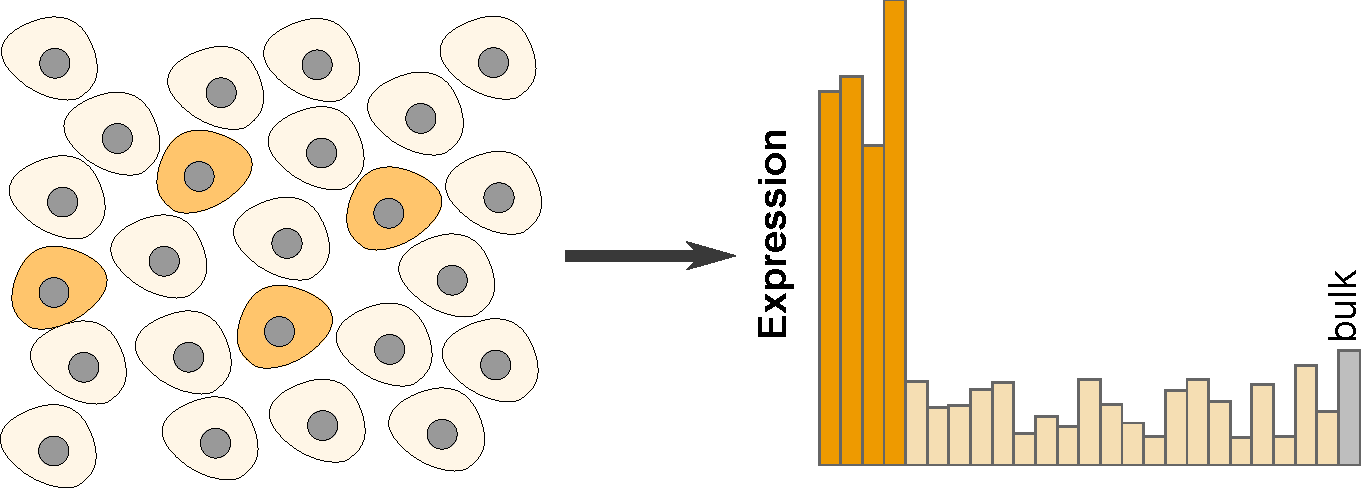
\includegraphics[width=0.6\linewidth]{figs/bulk_issue1.pdf}
    \item Dynamic effects are missed \\
      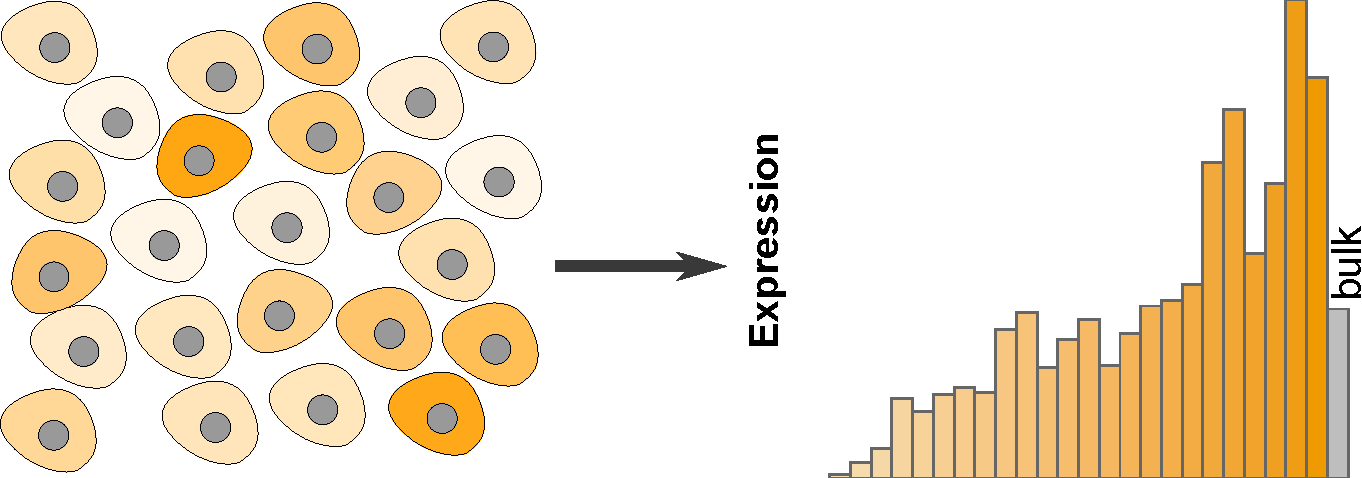
\includegraphics[width=0.6\linewidth]{figs/bulk_issue2.pdf}
  \end{itemize}
  
  \pause
  
  \textbf{Single-cell omics} generate one observation per cell, 
  unlocking new analytical tools
\end{frame}

%% Single-cell challenges
\begin{frame}[c]
  \frametitle{Single-cell challenges}
  
  \begin{itemize}
    \item Technical challenges: automation, minute sample amount, cost 
      per cell
    \item Computational challenges: big data, dropouts, noise, complex
      batch effects
    \item Conceptual challenges: what is a cell type? what is 
      biologically relevant? 
  \end{itemize}
  
  \vspace{0.5cm}
  \centering
  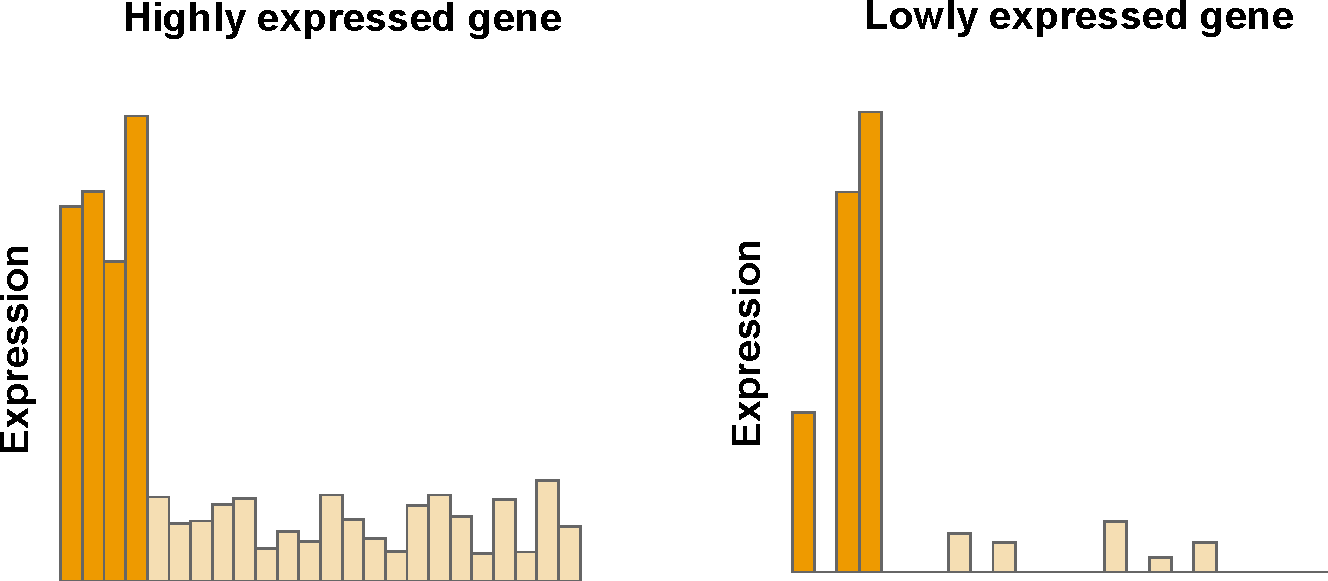
\includegraphics[width=0.8\linewidth]{figs/sc_issue.pdf}
\end{frame}

%% Proteomics vs transcriptomics
\begin{frame}[b]
  \frametitle{Proteomics vs transcriptomics}
  
  \begin{columns}
    \column{0.6\linewidth}
    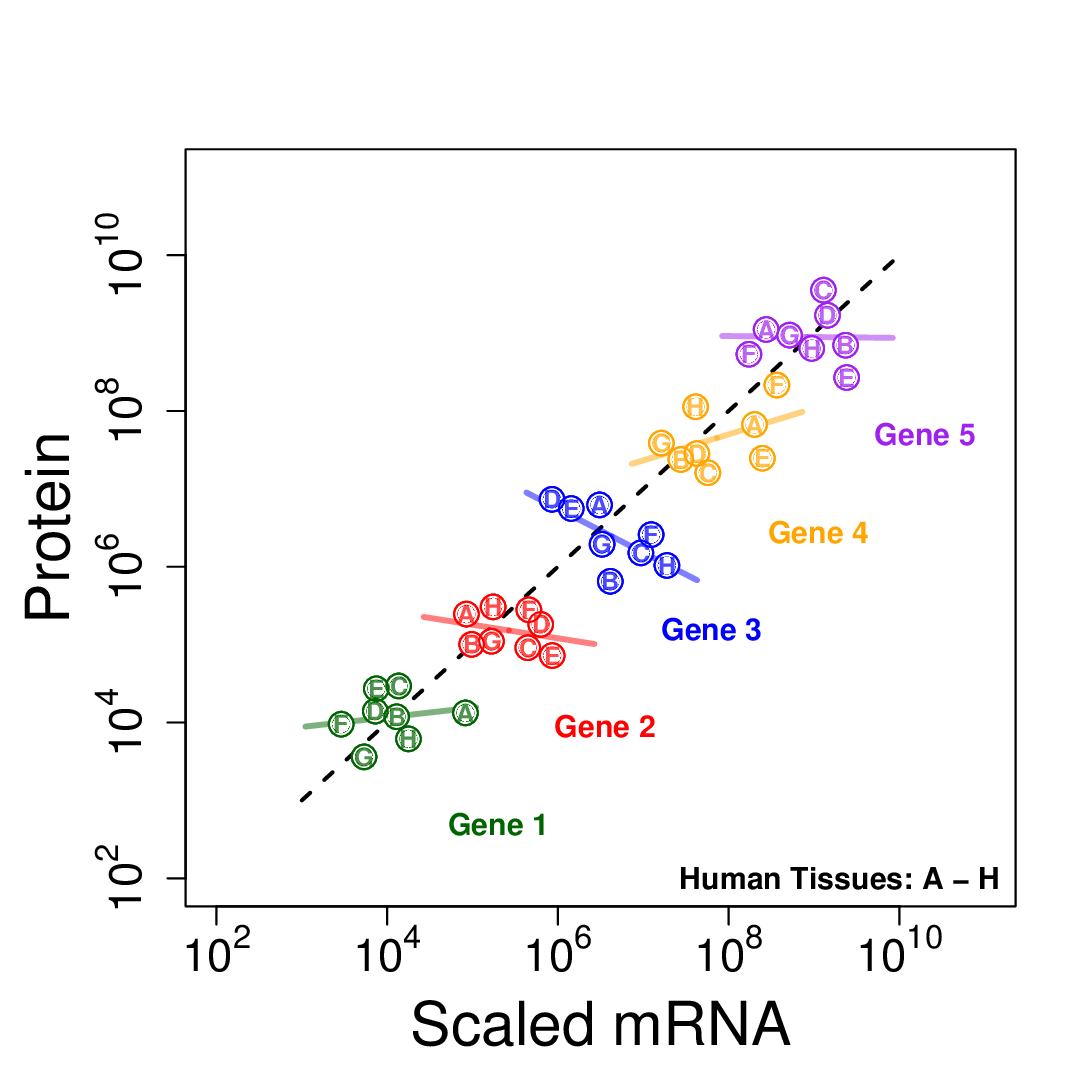
\includegraphics[width=\linewidth]{figs/simsons_paradox_in_gene_regulation.png}
    \column{0.4\linewidth}
    \centering
    \pause
    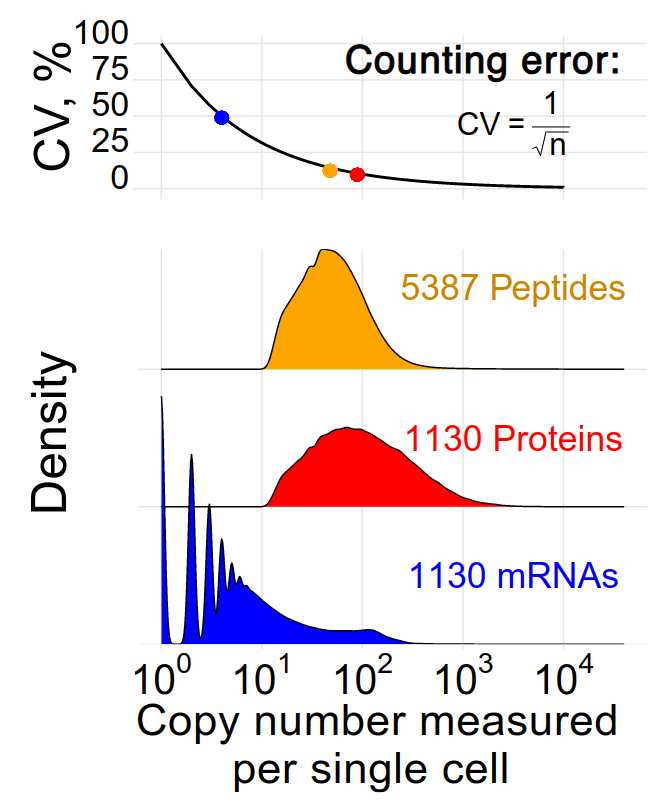
\includegraphics[width=\linewidth]{figs/Counting_error.png}
  
  \end{columns}
  
  \vfill
  \footnotesize
  Source: \cite{Franks2017-lo}, \cite{Specht2020-jm}.
  
\end{frame}


%% Single-cell proteomics
\begin{frame}
  \frametitle{Single-cell proteomics}
  
  Single-cell proteomics recently achieved a milestone by quantifying 
  > 1000 proteins for > 1000 single cells 
  {\footnotesize(\cite{Specht2020-jm})}. 

  \vfill
  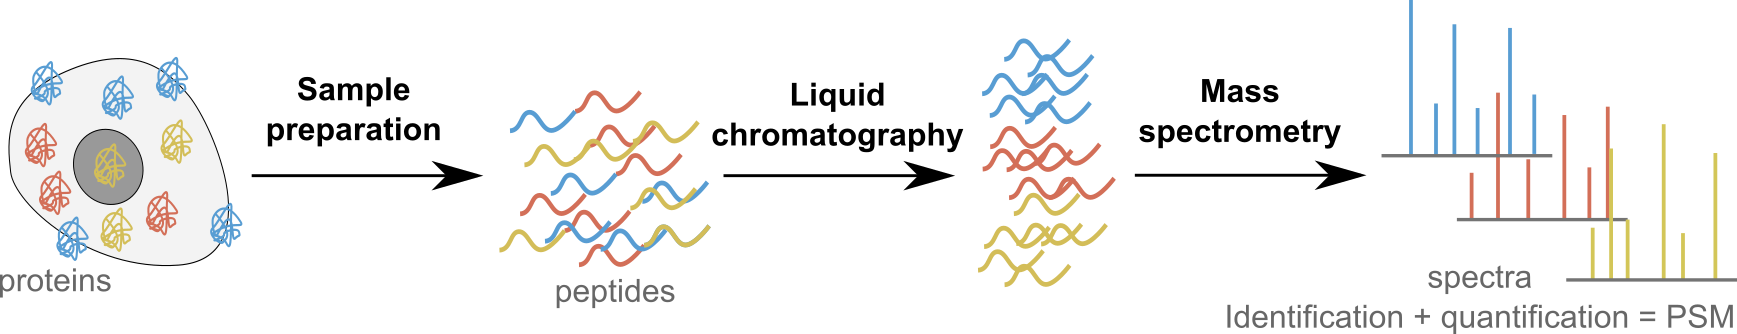
\includegraphics[width=\linewidth]{figs/MS-SCP.png}
  
  \vfill
  \begin{itemize}
    \item Label-free quantification: accurate quantification, but low 
      throughput and low identification rate
    \item Multiplexed: label cross contamination, but high throughput 
      and increased identification rate
  \end{itemize}

\end{frame}

%% Our contribution
\begin{frame}
  \frametitle{Our contribution}
  
  We offer a solution to the lack of good computational tools for 
  handling SCP data.

  \vfill
  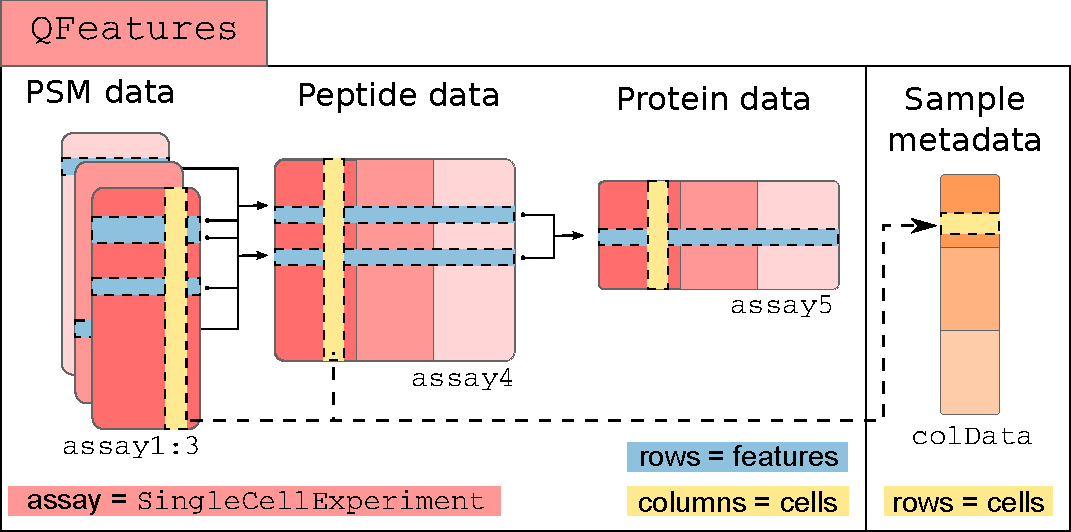
\includegraphics[width=0.8\linewidth]{figs/SCP_framework.pdf}
  
  \vfill
  \begin{itemize}
    \item \hcode{scpdata} disseminates curated SCP data sets 
    for method development and benchmarking
    \item \hcode{scp} implements functions to streamline the 
    analysis of SCP data
  \end{itemize}

\end{frame}


%% SCP pipeline
\begin{frame}[fragile]
  \frametitle{SCP pipeline}
 
  \begin{columns}
    \column{0.3\linewidth}
    \footnotesize
    \begin{enumerate}
      \item Input data
      \item QC on features
      \item QC on samples
      \item Peptide aggregation
      \item Log-normalization
      \item Feature selection
      \item Imputation
      \item Protein aggregation 
      \item Data integration
      \item Dimension reduction
    \end{enumerate}
    
    \column{0.8\linewidth}
    
    \begin{lstlisting}
readSCP(quantTable = quantData, 
        metaTable = metaData,
        channelCol = "Channel", 
        batchCol = "Set") %>%
  zeroIsNA(i = 1:4) %>%
  filterFeatures(~ Potential.contaminant != "+") %>%
  computeSCR(i = 1:4, 
             colDataCol = "SampleType",
             carrierPattern = "Carrier",
             samplePattern = "Monocyte") %>%
  filterFeatures(~ .meanSCR < 0.1) %>%
  subsetByAssay(dims(.)[1, ] > 150) %>%
  computeMedianCV(i = 1:3, 
                  proteinCol = "protein",
                  peptideCol = "peptide") %>%
  aggregateFeaturesOverAssays(i = 1:3, 
                              name = 4:6,
                              fcol = "peptide",
                              fun = robustSummary) %>%
  joinAssays(i = 4:6, name = "peptides") %>%
  normalize(i = "peptides", 
            method = "median", na.rm = TRUE) %>%
  logTransform(i = "normAssay",
               base = 2) %>%
  impute(i = "normAssay",
         method = "knn") %>%
  aggregateFeatures(i = "logAssay", 
                    name = "proteins",
                    fcol = "protein") ->
  scp
    \end{lstlisting}
  \end{columns}
\end{frame}



%% The SCoPE2 dataset
\begin{frame}[allowframebreaks]
  \frametitle{The SCoPE2 dataset}
  
  \vfill
  SCoPE2 dataset  {\footnotesize(\cite{Specht2020-jm})} = current 
  state-of-the-art SCP dataset 

  \vfill
  Replication of the analysis using \hcode{scp}:

  \vfill
  \begin{columns}
    \column{0.5\linewidth}
    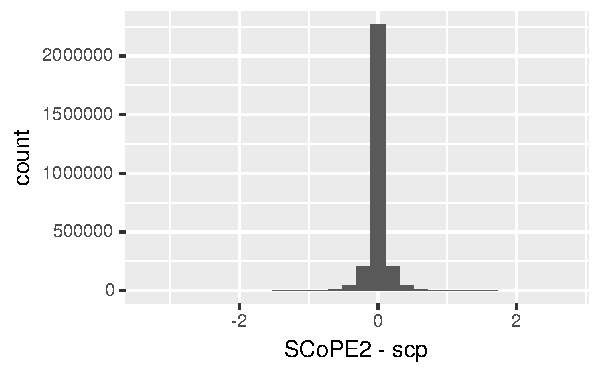
\includegraphics[width=\linewidth]{figs/Benchmark_prot_err.pdf}
    \column{0.5\linewidth}
    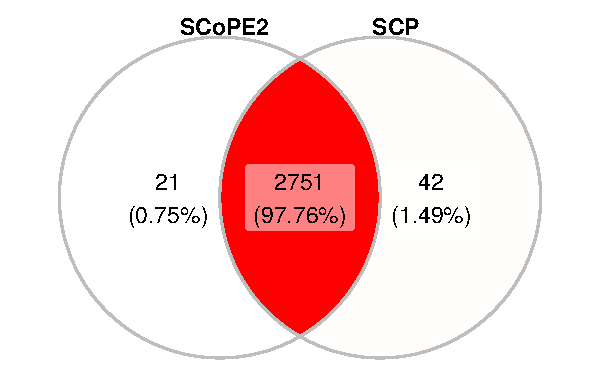
\includegraphics[width=\linewidth]{figs/Benchmark_prot_venn.pdf}
  \end{columns}
  
  \framebreak
  
  \vfill
  \begin{columns}
    \column{0.5\linewidth}
    SCoPE2\\
    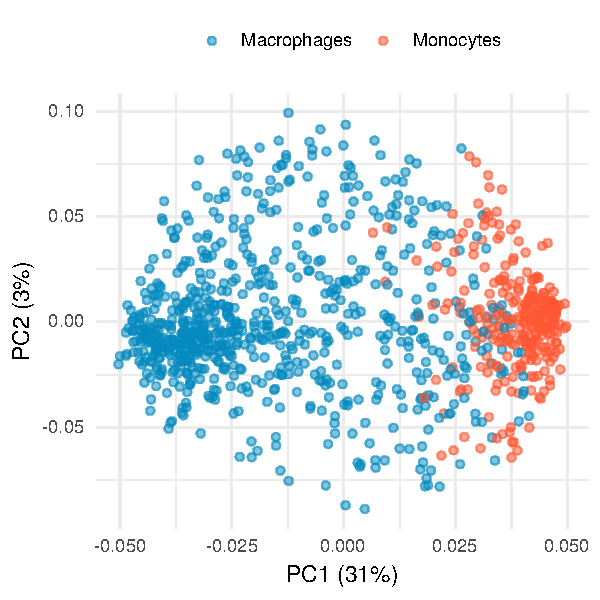
\includegraphics[width=\linewidth]{figs/wPCA_SCoPE2.pdf}
    \column{0.5\linewidth}
    \hcode{scp}\\
    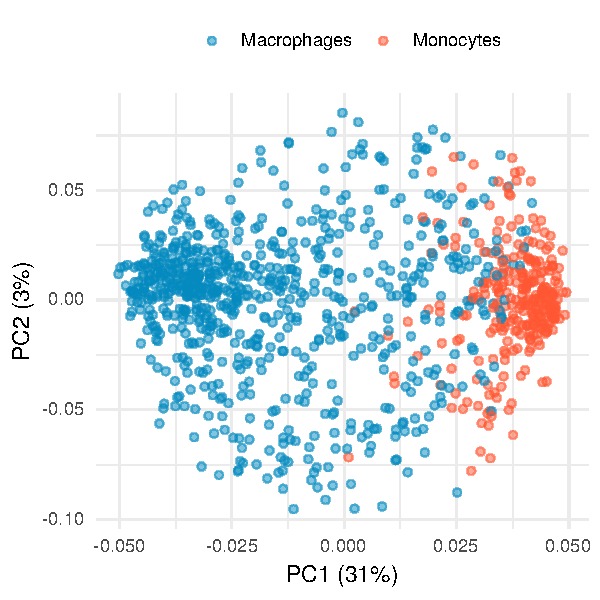
\includegraphics[width=\linewidth]{figs/wPCA_scp.pdf}
  \end{columns}
\end{frame}

%% Replication: conclusion
\begin{frame}
  \frametitle{Replication: conclusion}
  
  \hcode{scp} provides a standardized pipeline for unified and 
  reproducible analysis of SCP data:
  
  \vfill
  \begin{enumerate}
    \item SCoPE2 ({\footnotesize \cite{Specht2020-jm}}): almost 
      perfect replication, new metrics included in \hcode{scp}, 
      highlighted issues and possible improvements 
    \item Trajectory analysis on chicken utricle ({\footnotesize 
      \cite{Zhu2019-ja}}): lack of good documentation
  \end{enumerate}
  
  \vfill
  This demonstrate the successful application of our software to 
  various SCP datasets. 
  
\end{frame}

%% SCP challenges: batch effect
\begin{frame}
  \frametitle{SCP challenges: batch effect}
  
  \begin{columns}
    \column{0.5\linewidth}
    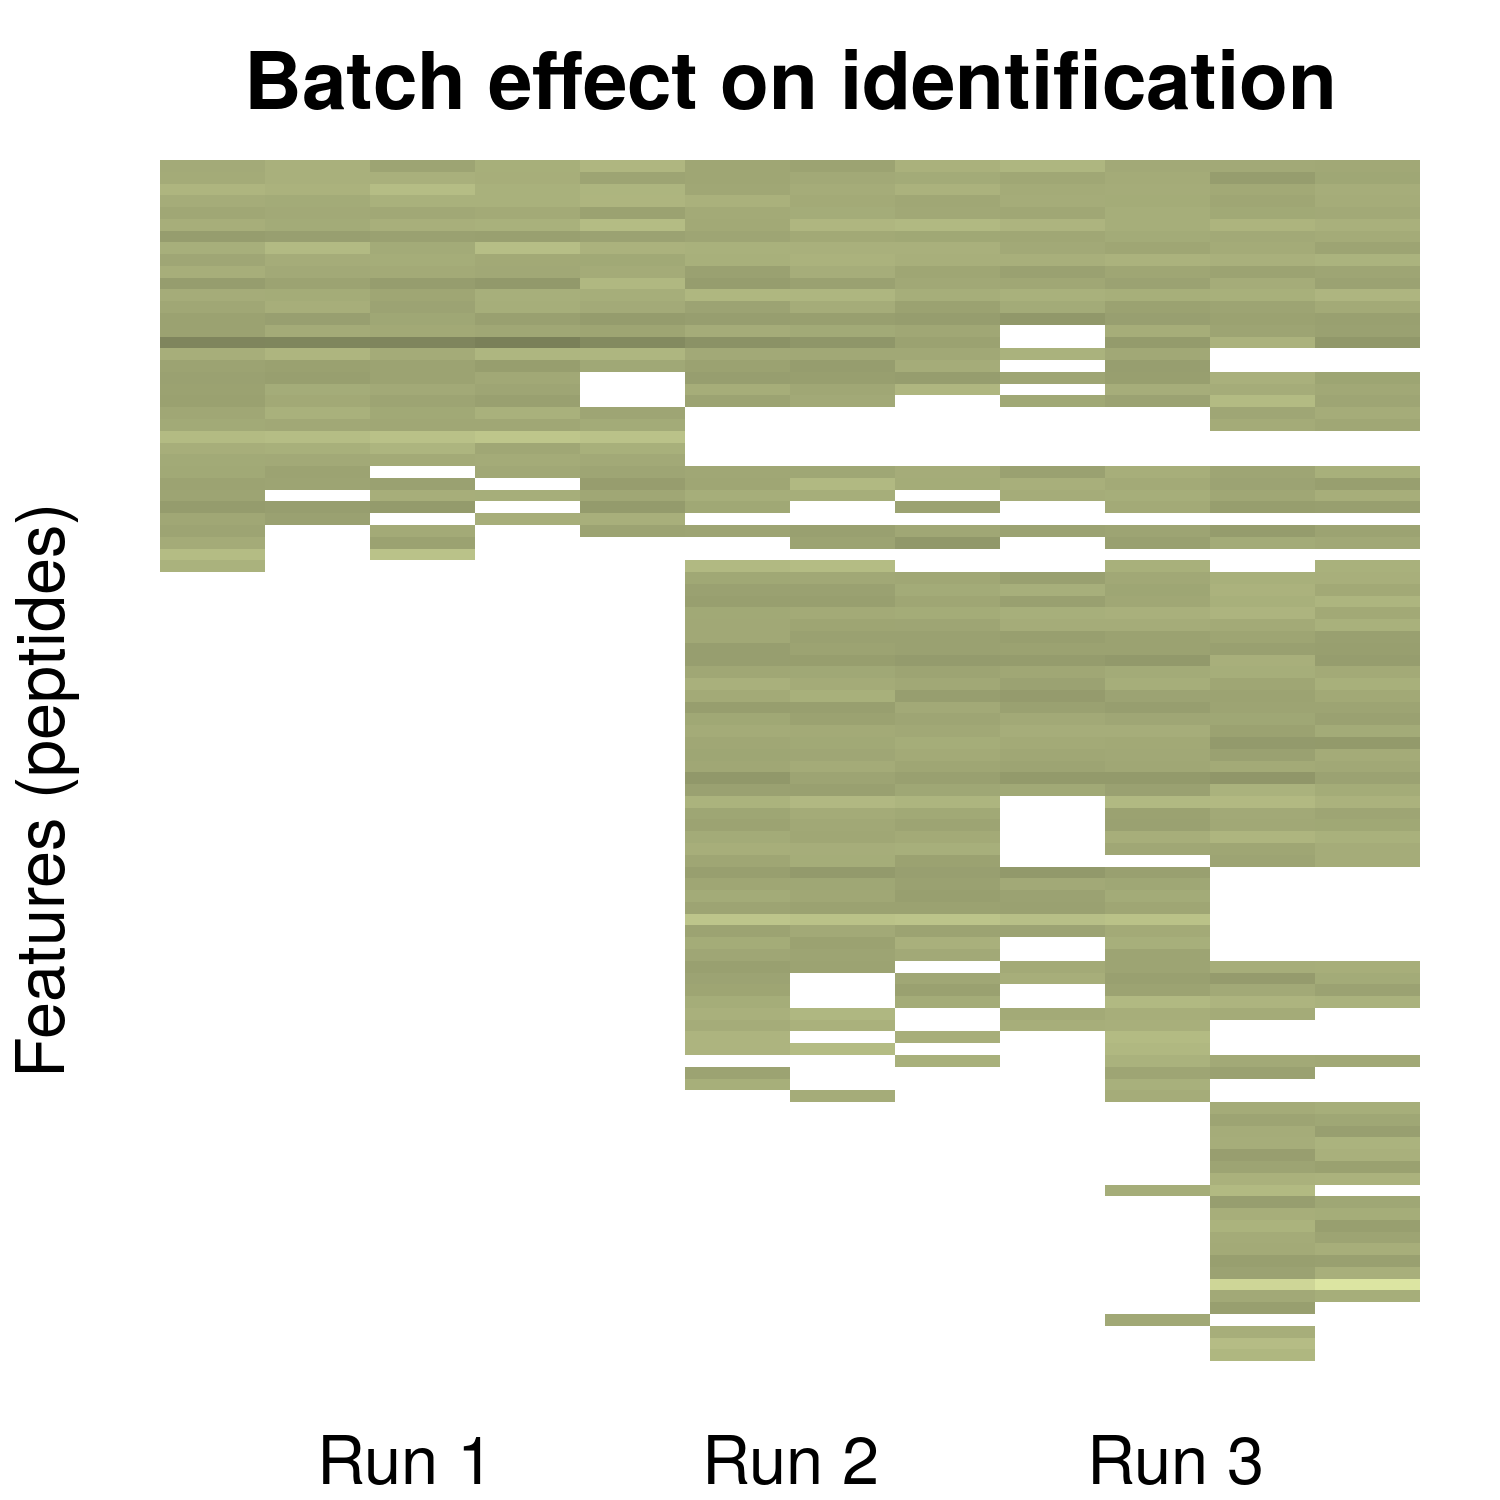
\includegraphics[width=\linewidth]{figs/batch_effects.png}
    \column{0.5\linewidth}
    \vspace{1cm}
    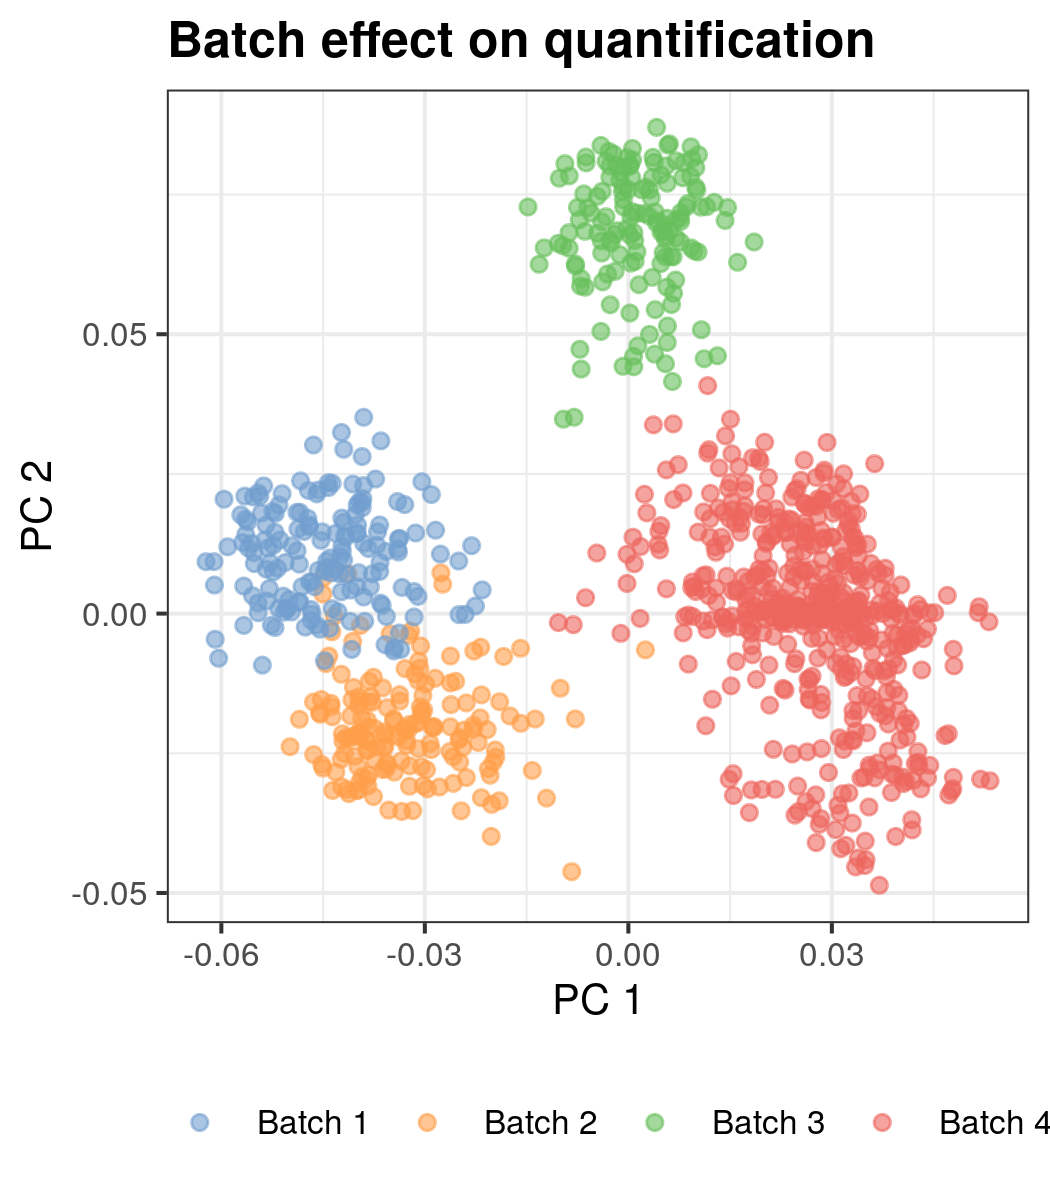
\includegraphics[width=\linewidth]{figs/PCA_batch_effect.png}
  \end{columns}
  
\end{frame}

%% SCP challenges: missingness
\begin{frame}
  \frametitle{SCP challenges: missingness}
  
  \begin{columns}
    \column{0.4\linewidth}
    \begin{itemize}
      \item Biological missingness
      \item Technical missingness
      \item Both
    \end{itemize}
    \column{0.7\linewidth}
    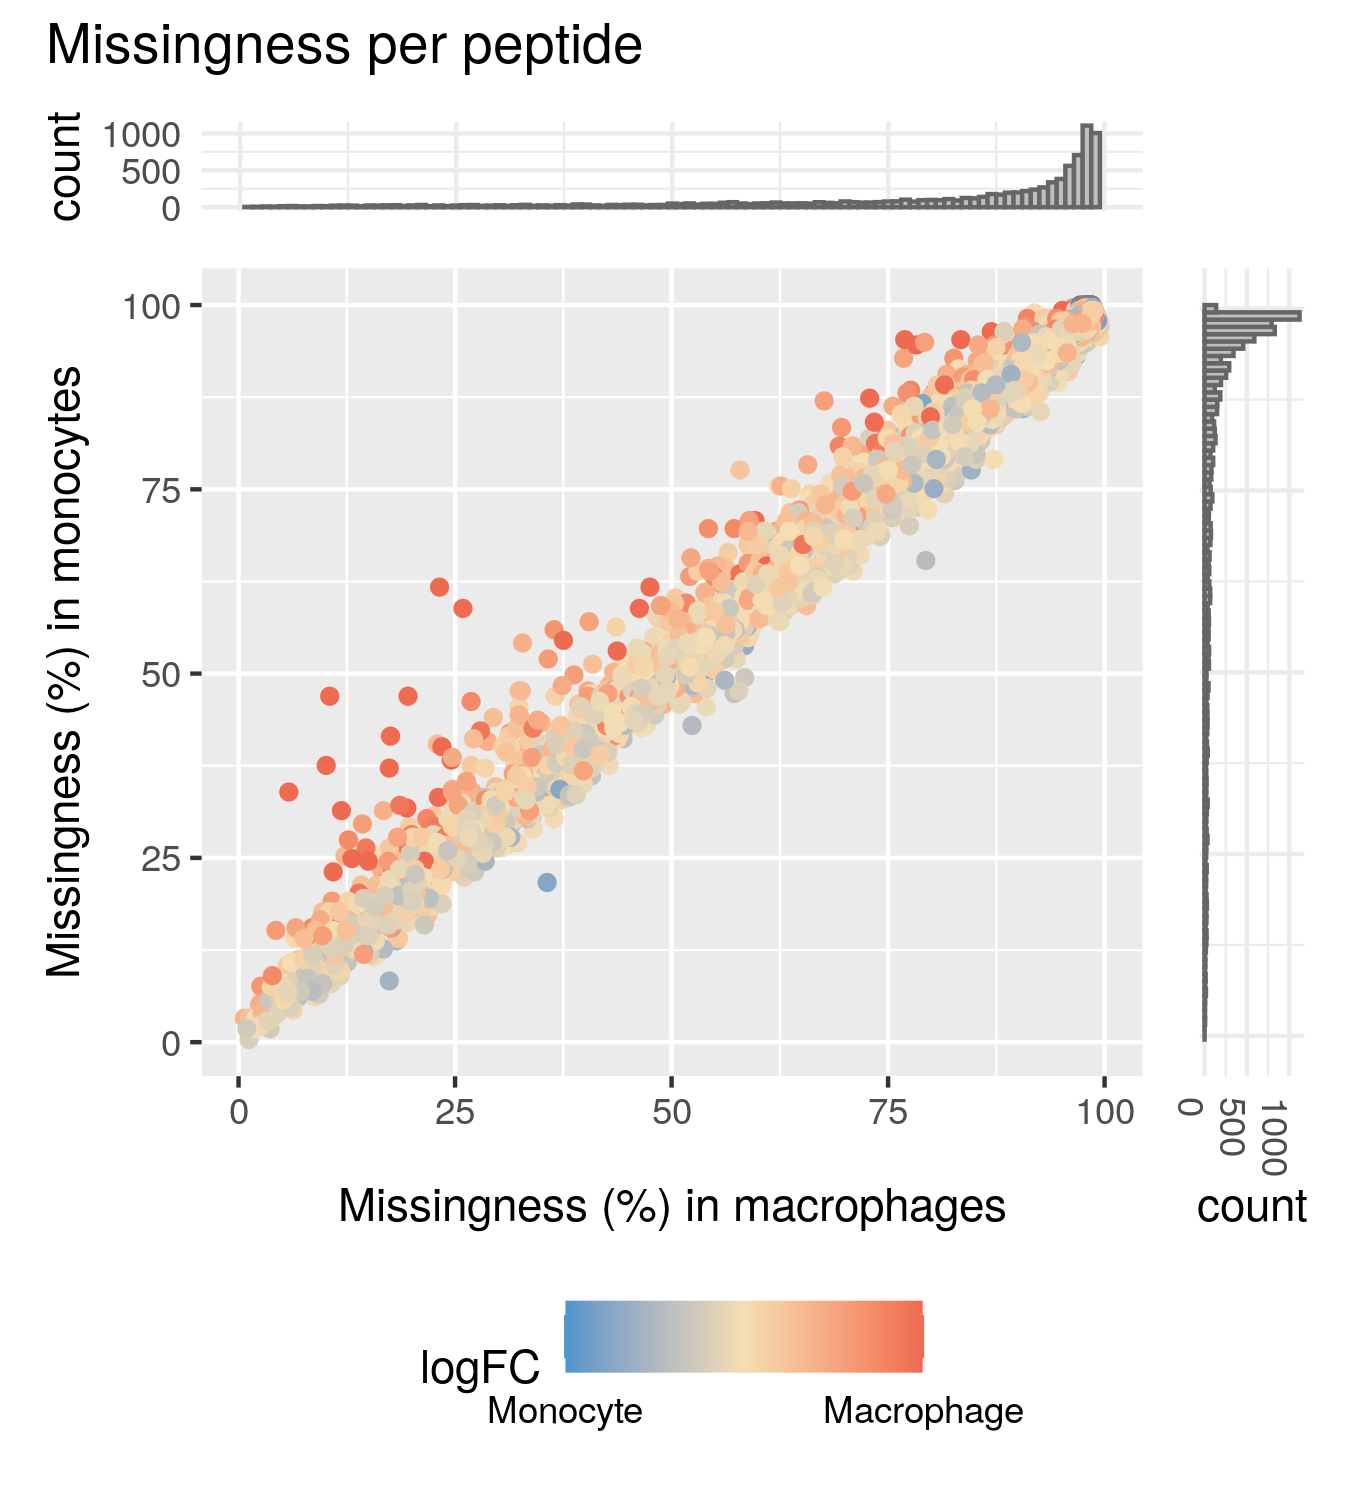
\includegraphics[width=\linewidth]{figs/missing_peptide.png}
  \end{columns}
  
\end{frame}


%% SCP challenges: data modeling
\begin{frame}
  \frametitle{SCP challenges: data modeling}
  
  \textbf{Hurdle model} {\scriptsize (\cite{Goeminne2020-op})}
  
  \vfill
  \centering
  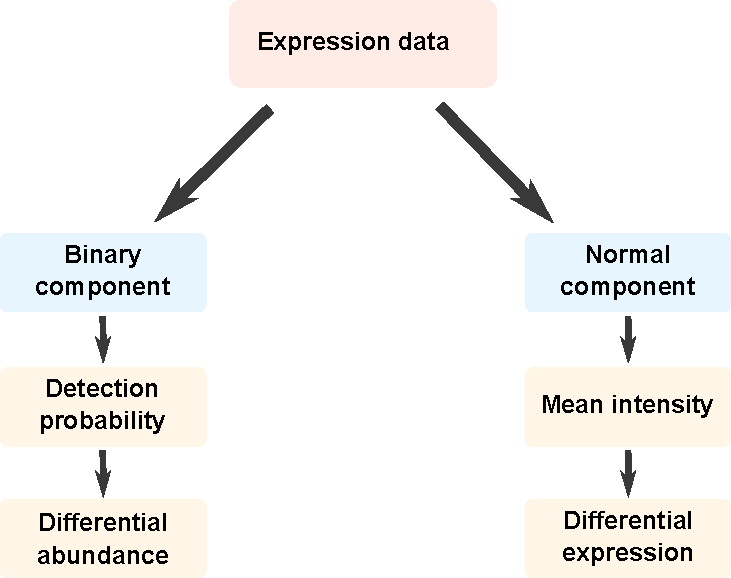
\includegraphics[width=0.7\linewidth]{figs/hurdle.pdf}
  
\end{frame}

%% Takehome message
\begin{frame}
  \frametitle{Takehome message}
  
  \begin{itemize}
    \item SCP is an emerging but very promosing field!
    \item We developed a computational infrastructure to formalize SCP
      data analyses
    \item The infrastructure could be applied to reproduce 2 published 
      analyses
    \item Exciting challenges are yet to be solved
  \end{itemize}
  
\end{frame}

%% Acknowledgements
\begin{frame}[b]
  \frametitle{Acknowledgements}
  \centering
  
  Many thanks to my promoter \textbf{Pr. Laurent Gatto}
  
  \vfill
  Thanks you for your attention!

  {\footnotesize I'm happy to take questions now or at the discussion 
  tables}
  
  \vfill
  \begin{columns}
    \column{0.1\linewidth}
    
\includegraphics[width=\linewidth]{figs/eurobioc2020.jpg}
    \column{0.9\linewidth}
    See you at the EuroBioc2020 (online) 
  \end{columns}
  
  \vfill
  \begin{columns}
    \column{0.4\linewidth}
    
\includegraphics[width=\linewidth]{figs/ucl.png}
    \column{0.4\linewidth}
    \column{0.2\linewidth}
    
\includegraphics[width=\linewidth]{figs/fnrs.png}
  \end{columns}
\end{frame}



%-----------------------------------------------
% References
%-----------------------------------------------

\begin{frame}[allowframebreaks]{References}
  \scriptsize
  \bibliographystyle{plainnat}
  \bibliography{ref}
\end{frame}


\end{document}
